%!TEX root = ../main.tex

\chapter{Machine Learning}\label{cha:machinelearning}

In this chapter a new approach to identifying strategies that are the same will be presented.
A new type of tournament will be presented, and the summary of the results of this tournament will then be used to train a Machine Learning model.
The model is then able to predict whether new strategies are the same as ones already implemented within Axelrod-Python.

\section{Ashlock Tournament}\label{sec:ashlock_tourn}
An Ashlock tournament is where all strategies entered play against a probe strategy for a range of parameters, and do not play each other.
A results file is then created with information about how the strategies performed and behaved in the tournament.

%TODO, example row from dataframe of results




\section{Training the model}\label{sec:training_model}

To train the model, all strategies available in Axelrod-Python were entered into an Ashlock tournament.
T

A new table can then be produced where the results of each strategies are compared.
Given two strategies $A$ and $B$, they have a set of variables $\{x_1^{(A)}, x_2^{(A)}, \dots, x_n^{(A)}\}$ or $\{x_1^{(B)}, x_2^{(B)}, \dots, x_n^{(B)}\}$ which are taken from the results file.
To compare the strategies, a new set of variables $\{r_1, r_2, \dots, r_n \}$ is created where:
$$
r_k = \frac{\min(x_k^{(A)}, x_k^{(B)})}{\max(x_k^{(A)}, x_k^{(B)})}.
$$
In the case where $x_k^{(A)} = x_k^{(B)} = 0$, the ratio $r_k$ is set to 1 as the two variables are equal.
By comparing the names of the two strategies, a new column can be added to the data containing a boolean variable where a value of 1 implies that the two strategies are the same, and 0 if they are different.


\section{Initial Results}

\begin{figure}[tb]
    \centering
    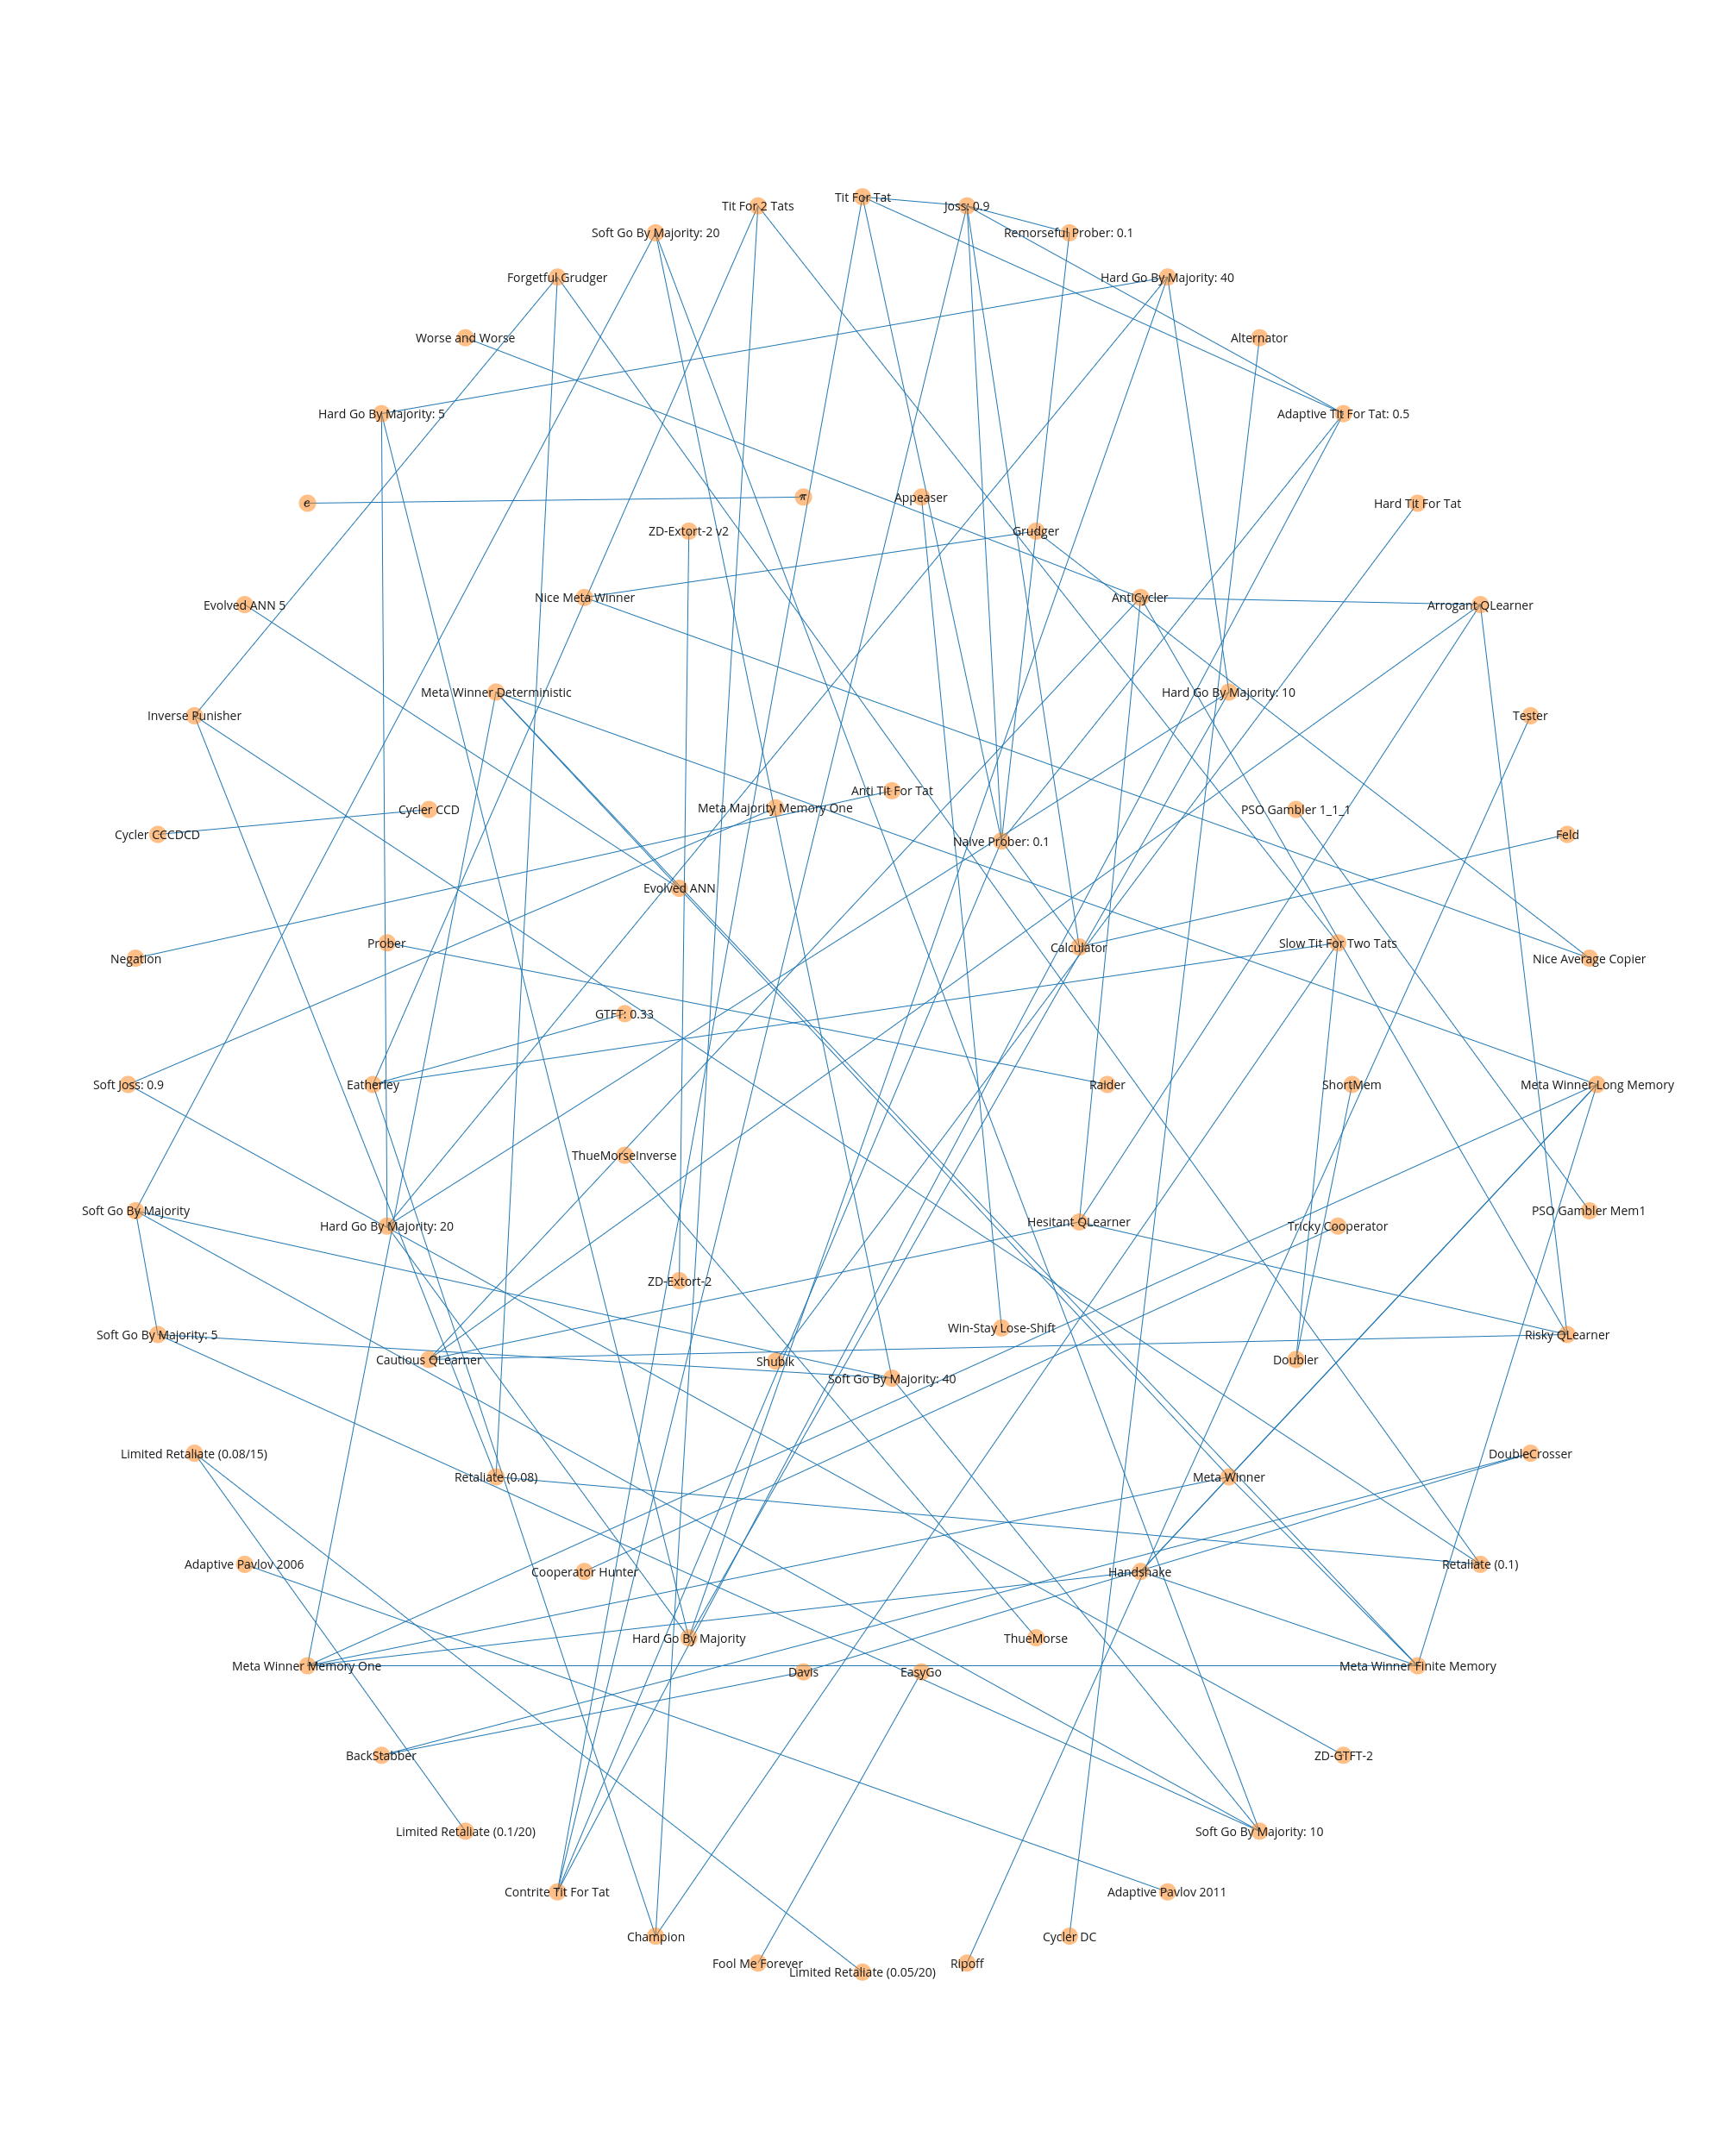
\includegraphics[width=\linewidth]{../img/neighbourhoods/overall.png}
    \caption{Caption here}
    \label{fig:figure1}
\end{figure}

\begin{figure}[htbp!]
\subfloat[]{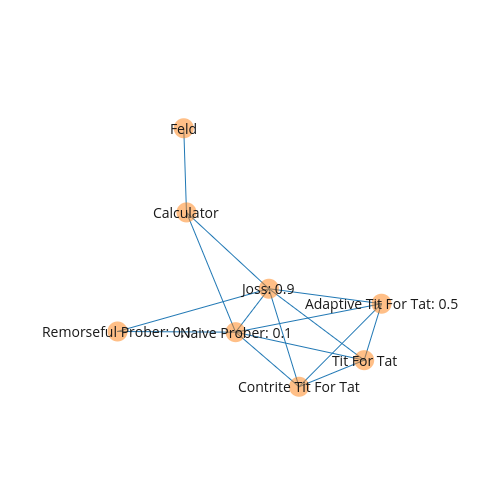
\includegraphics[width = 0.3\textwidth]{../img/neighbourhoods/1.png}}
\subfloat[]{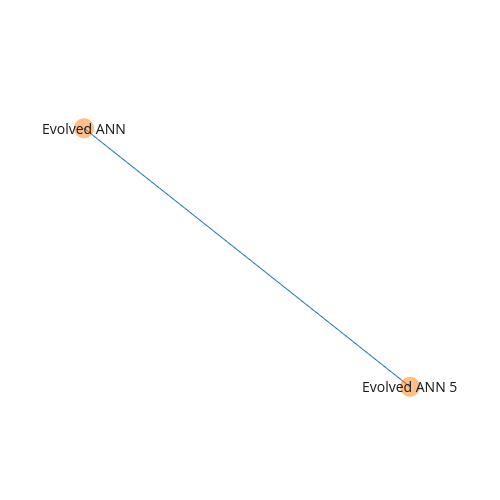
\includegraphics[width = 0.3\textwidth]{../img/neighbourhoods/2.png}}
\subfloat[]{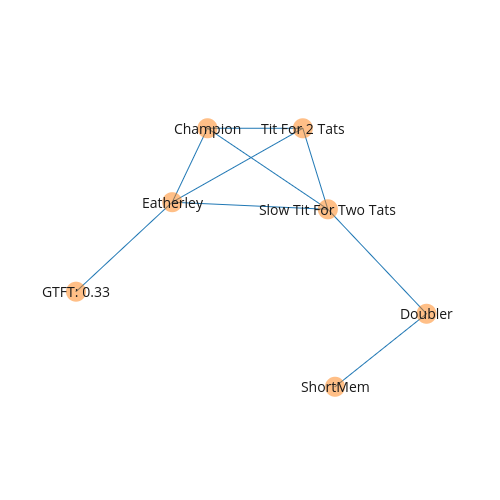
\includegraphics[width = 0.3\textwidth]{../img/neighbourhoods/3.png}} \\
\end{figure}
\begin{figure}[htbp!]
\ContinuedFloat
\subfloat[]{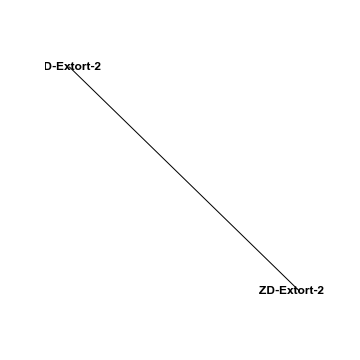
\includegraphics[width = 0.3\textwidth]{../img/neighbourhoods/4.png}}
\subfloat[]{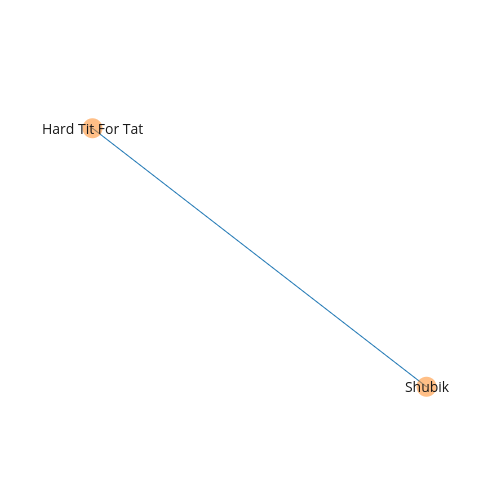
\includegraphics[width = 0.3\textwidth]{../img/neighbourhoods/5.png}}
\subfloat[]{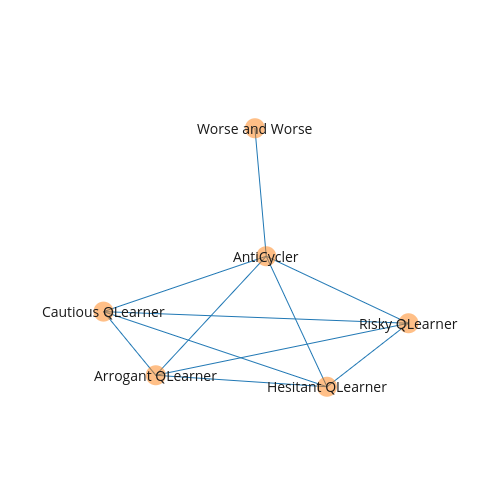
\includegraphics[width = 0.3\textwidth]{../img/neighbourhoods/6.png}} \\
\end{figure}
\begin{figure}[htbp!]
\ContinuedFloat
\subfloat[]{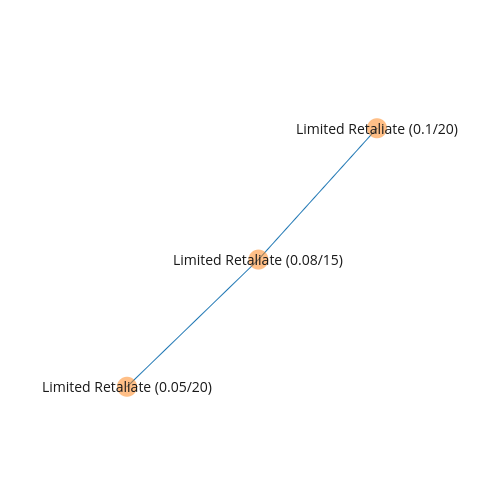
\includegraphics[width = 0.3\textwidth]{../img/neighbourhoods/7.png}}
\subfloat[]{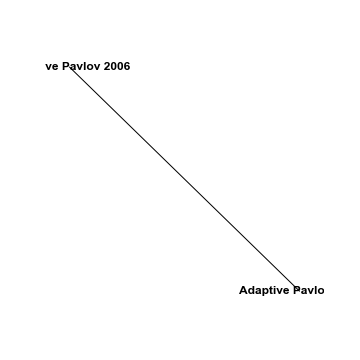
\includegraphics[width = 0.3\textwidth]{../img/neighbourhoods/8.png}}
\subfloat[]{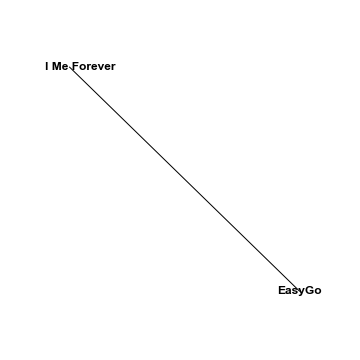
\includegraphics[width = 0.3\textwidth]{../img/neighbourhoods/9.png}} \\
\end{figure}
\begin{figure}[htbp!]
\ContinuedFloat
\subfloat[]{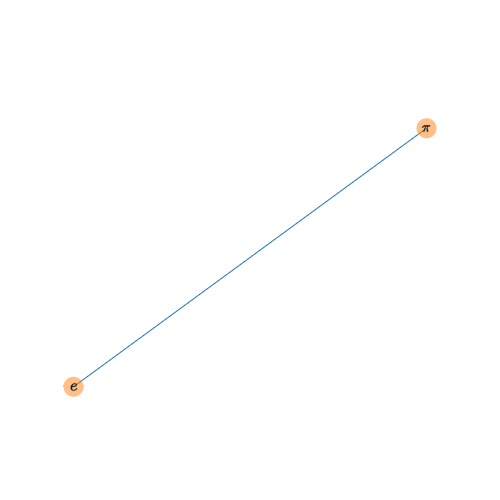
\includegraphics[width = 0.3\textwidth]{../img/neighbourhoods/10.png}}
\subfloat[]{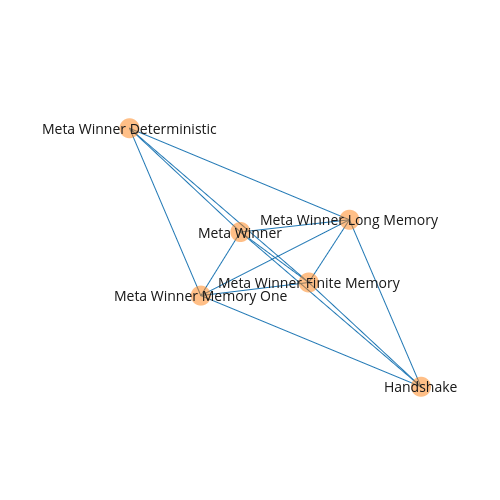
\includegraphics[width = 0.3\textwidth]{../img/neighbourhoods/11.png}}
\subfloat[]{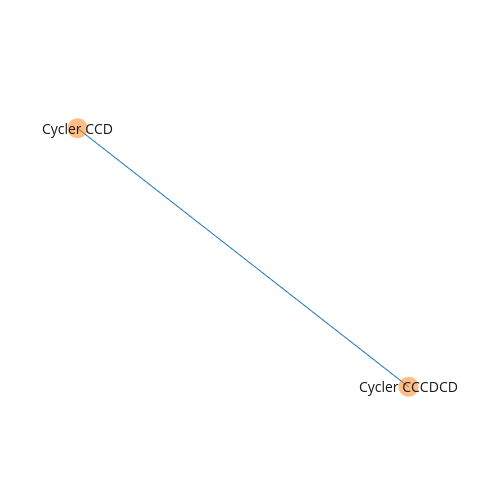
\includegraphics[width = 0.3\textwidth]{../img/neighbourhoods/12.png}} \\
\end{figure}
\begin{figure}[htbp!]
\ContinuedFloat
\subfloat[]{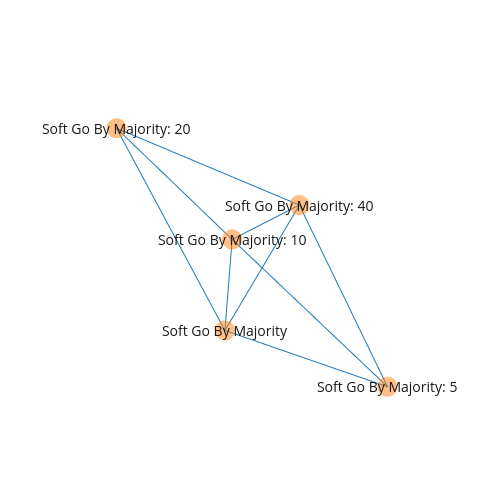
\includegraphics[width = 0.3\textwidth]{../img/neighbourhoods/13.png}}
\subfloat[]{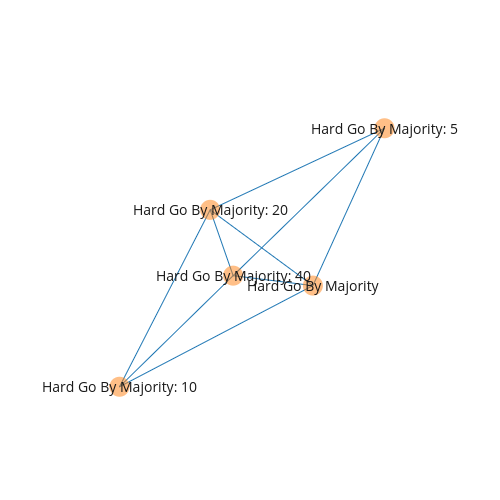
\includegraphics[width = 0.3\textwidth]{../img/neighbourhoods/14.png}}
\subfloat[]{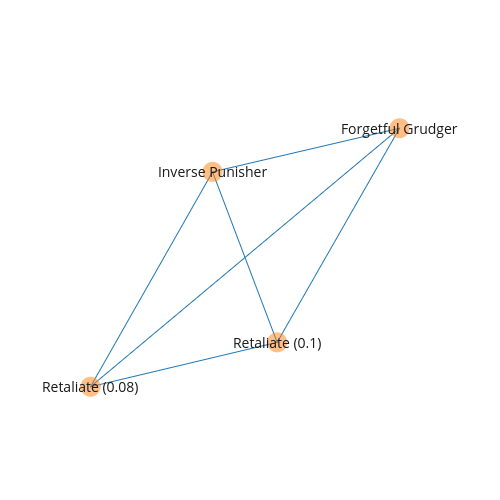
\includegraphics[width = 0.3\textwidth]{../img/neighbourhoods/15.png}} \\
\end{figure}
\begin{figure}[htbp!]
\ContinuedFloat
\subfloat[]{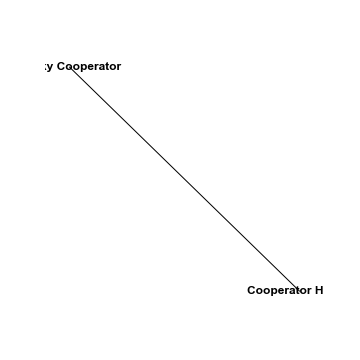
\includegraphics[width = 0.3\textwidth]{../img/neighbourhoods/16.png}}
\subfloat[]{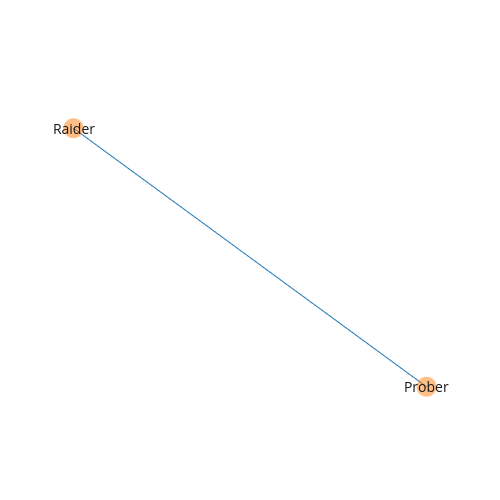
\includegraphics[width = 0.3\textwidth]{../img/neighbourhoods/17.png}}
\subfloat[]{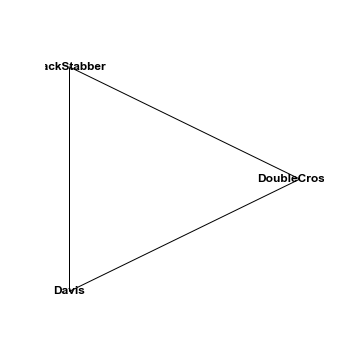
\includegraphics[width = 0.3\textwidth]{../img/neighbourhoods/18.png}} \\
\end{figure}
\begin{figure}[htbp!]
\ContinuedFloat
\subfloat[]{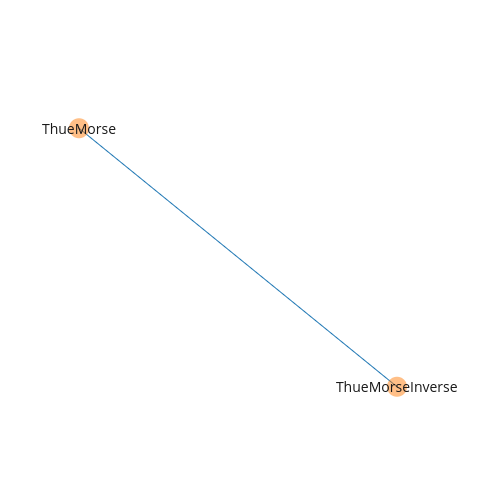
\includegraphics[width = 0.3\textwidth]{../img/neighbourhoods/19.png}}
\subfloat[]{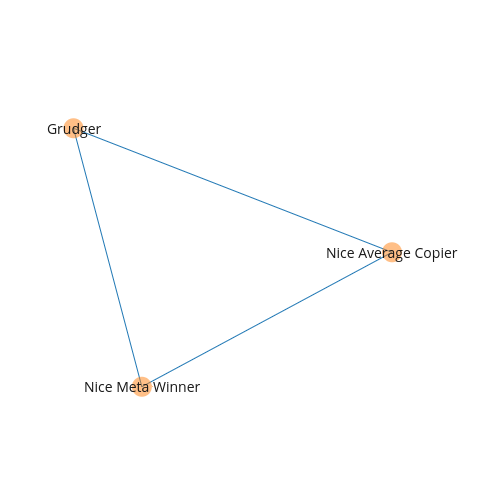
\includegraphics[width = 0.3\textwidth]{../img/neighbourhoods/20.png}}
\subfloat[]{
\includegraphics[width = 0.3\textwidth]{../img/neighbourhoods/21.png}} \\
\end{figure}
\begin{figure}[htbp!]
\ContinuedFloat
\subfloat[]{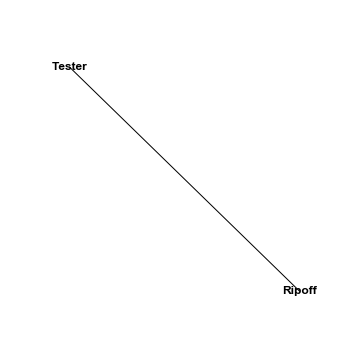
\includegraphics[width = 0.3\textwidth]{../img/neighbourhoods/22.png}}
\subfloat[]{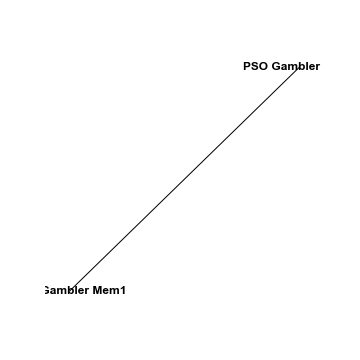
\includegraphics[width = 0.3\textwidth]{../img/neighbourhoods/23.png}}
\subfloat[]{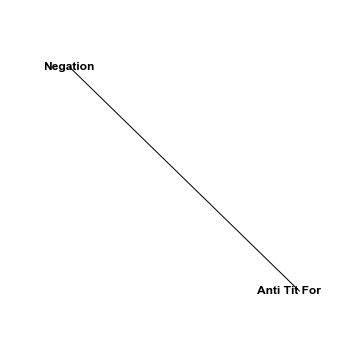
\includegraphics[width = 0.3\textwidth]{../img/neighbourhoods/24.png}} \\
\end{figure}
\begin{figure}[htbp!]
\ContinuedFloat
\subfloat[]{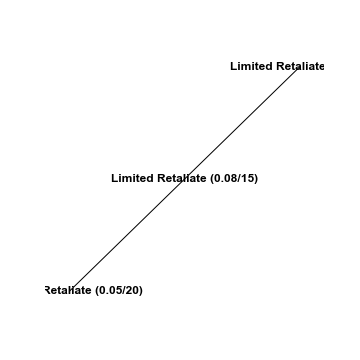
\includegraphics[width = 0.3\textwidth]{../img/neighbourhoods/25.png}}
\subfloat[]{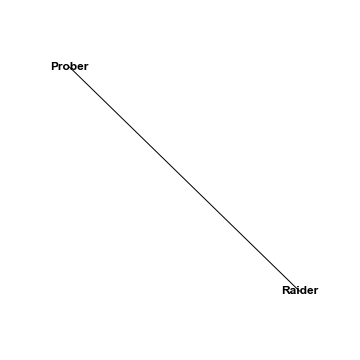
\includegraphics[width = 0.3\textwidth]{../img/neighbourhoods/0.png}}\\
\end{figure}
